Inverse AC Josephson effect and some BCS questions.

\begin{parts}
	\part Properties of SC:
	\begin{enumerate}
		\item Zero resistivity under critical temperature $T_\textnormal{c}$.
		\item Meissner effect: $\chi = -1$ and SC repels all applied field less than the critical field.
	\end{enumerate}
	
	Sketch of resistivity $\rho$ against temperature $T$:
	\begin{figure}[H]
		\centering
		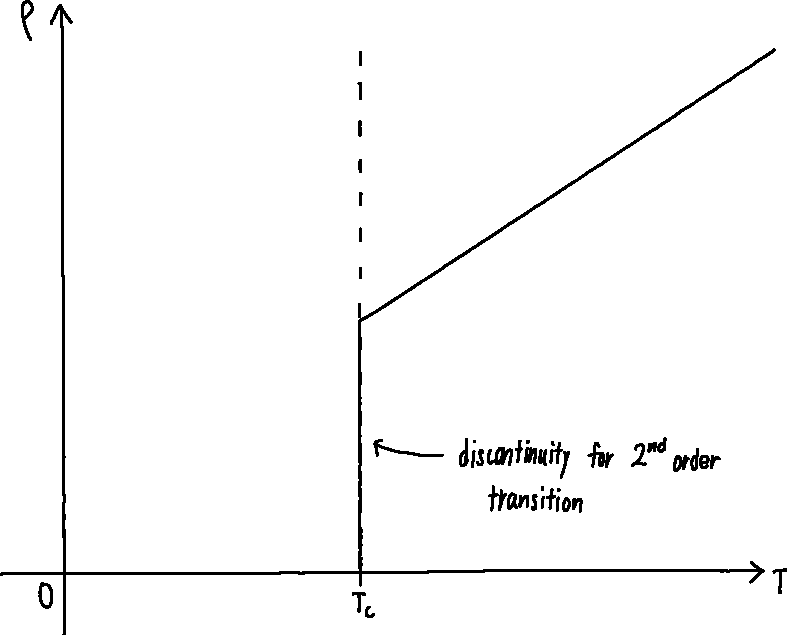
\includegraphics[width=.7\linewidth]{q5-resistivity}
	\end{figure}
	
	For BCS SC, below $T < T_\textnormal{c}$, the Fermi surface destabilises into a gap due to the electrons forming a BCS condensate in terms of Cooper pairs via the electron-phonon interaction.
	
	\part 1st Josephson equation: $I(\phi) = I_J \sin\phi$
	
	2nd Josephson equation: $V = \dfrac{\hbar}{2e} \pdderi{\phi}{t}$
	
	For an AC current,
	\begin{align*}
		V &= V_0 + V_\textnormal{rf} \cos\omega t \\
		\phi(t) &= \phi_0 + \frac{2eV_0}{\hbar} t + \frac{2eV_\textnormal{rf}}{\hbar\omega} \sin\omega t \\
		\Rightarrow I(t) &= I_J \sin\sbracket{\phi_0 + \frac{2eV_0}{\hbar} t + \frac{2eV_\textnormal{rf}}{\hbar\omega} \sin\omega t} \\
		&= I_J \sum_{n = -\infty}^{\infty} \rbracket{-1}^n J_n\rbracket{\frac{2eV_\textnormal{rf}}{\hbar\omega}} \sin\sbracket{\phi_0 + \underbracket{\frac{2eV_0}{\hbar} t - n\omega t}_{\rbracket{2eV_0 / \hbar - n\omega}t}}
	\end{align*}
	
	For every $n\omega = \dfrac{2eV_0}{\hbar}$, the time dependence of $I$ vanishes $\Rightarrow$ DC spikes (Shapiro steps) develop.
	This is called the inverse AC Josephson effect.
	
	In the presence of microwaves, due to the inverse AC effect, we have a series of Shapiro steps.
	For the graph without microwaves, we have a voltage biased JJ: the jump in the middle is due to the breakdown of Cooper pairs and voltage develops as a consequence of the presence of normal state electrons $\Rightarrow$ finite $R$.
	
	The reason why the jump in current is different is due to the RF voltage reducing $I_J$ via the Bessel sum.
	
	We have $I_J \simeq \SI{0.1}{\milli\ampere}$ and $\omega \simeq 2eV_0 / \hbar = 2e/\hbar \rbracket{\SI{2.05}{\milli\volt}} = \SI{6.23e12}{\radian\per\second}$.
	
	\part Condensation energy: $E_\textnormal{cond} = \dfrac{B_\textnormal{c}^2}{2\mu_0} = g_n - g_s$ where $g_n$ and $g_s$ are the Gibbs free energy per unit volume associated to the normal and SC phases.
	
	Noting that $g = u - Ts + mB$, we have:
	\begin{align*}
		\inftsml{g} &= -s \inftsml{T} + B \inftsml{m} \\
		\Rightarrow \textnormal{Entropy\hspace{1em}} s &=
		-\rbracket{
		 \pderi{g}{T}
		}_B \\
		\Rightarrow \textnormal{Heat capacity\hspace{1em}} c &=
		\rbracket{
		 \pderi{u}{T}
		}_B \\
		&= T
		\rbracket{
		 \pderi{s}{T}
		}_B
		\textnormal{\hspace{1em}for $\inftsml{u} = T \inftsml{s} - m \inftsml{B}$} \\
		&= -T
		\rbracket{
		 \pdiff{T}
		 \rbracket{
		  \pderi{g}{T}
		 }_B
		}_B
	\end{align*}
	
	Hence the jump in heat capacity:
	\begin{gather*}
		\Delta c = -T
		\sbracket{
		 \pdiff{T}
		 \rbracket{
		  \pderi{(\Delta g)}{T}
		 }_B
		}_B \\
		= -\frac{T B_0^2}{2 \mu_0}
		\sbracket{
		 \pdiff{T}
		 \rbracket{
		  \pdiff{T}
		  \rbracket{1 - \alpha t^2 + \beta t^3}^2
		 }_B
		}_B
		\textnormal{\hspace{1em}where $\alpha = \num{1.211}$, $\beta = \num{.211}$, $t = T/T_\textnormal{c}$}\\
		= -\frac{T B_0^2}{T_\textnormal{c}^2 \mu_0}
		\sbracket{
		 \rbracket{1 - \alpha t^2 + \beta t^3}
		 \rbracket{-2\alpha + 6\beta t}
		 + \rbracket{-2\alpha t^2 + 3\beta t^2}^2
		}\\
		= \SI{-616}{\joule\per\kelvin\per\metre\cubed}
		\textnormal{\hspace{1em}at $T=T_\textnormal{c} \Rightarrow t=1$}
	\end{gather*}
	
	\part From BCS, $\Delta C = 1.43 C_n$, and $C_n = \gamma T = \SI{317}{\joule\per\kelvin\per\metre\cubed}$, thus $\Delta C = \SI{450}{\joule\per\kelvin\per\metre\cubed}$.
	
	\part From BCS, $\abs{\Delta (0)} = 2\hbar\omega_\textnormal{D} \mathrm{e}^{-1/\lambda}$ and $k_\textnormal{B} T_\textnormal{c} \simeq 1.13 \hbar\omega_\textnormal{D} \mathrm{e}^{-1/\lambda}$:
	\begin{align*}
		k_\textnormal{B} T_\textnormal{c} &\simeq 1.13 \frac{\Delta}{2} \\
		\Delta &\simeq \frac{k_\textnormal{B} T_\textnormal{c}}{2.26} \\
		&= \SI{1.42e-4}{\electronvolt}
	\end{align*}
	
	Sketch of SC gap against temperature:
	\begin{figure}[H]
		\centering
		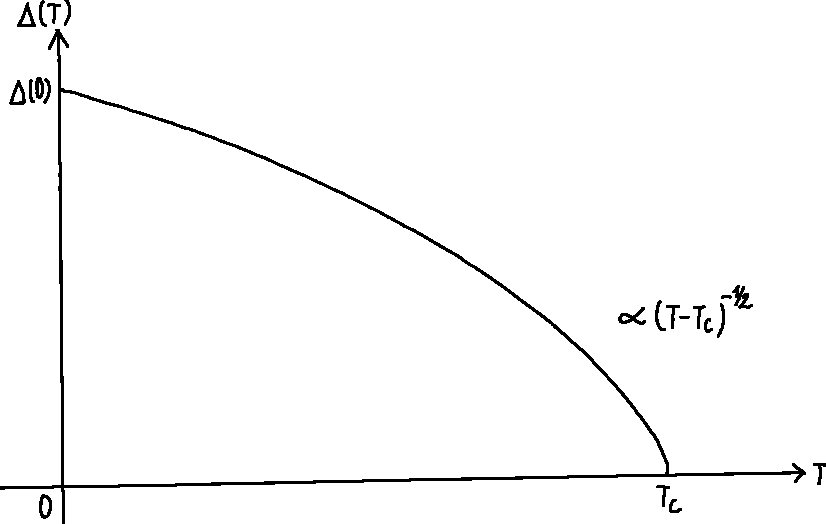
\includegraphics[width=.7\linewidth]{q5-energy-gap}
	\end{figure}
	As the gap is the result of the electrons at the Fermi surface delocalising to join the Cooper pair condensate, higher density should lead to larger gap.
\end{parts}